\chapter{Model evaluation} \label{ch:model_evaluation}

The fifth phase of CRISP-DM process model for data mining projects is evaluation;
this chapter presents the evaluation of results of the machine learning workflow to classify land use that was introduced in chapter~\ref{ch:ml_workflow};
classification algorithms described in section~\ref{sec:model_selection} were tested on the augmented Teranet dataset, production of which was described in chapter~\ref{ch:data_preparation}.
As was discussed in section~\ref{sec:model_selection}, no single classifier works better than others across all possible scenarios, and thus it is important to compare the performance of several classification algorithms on a given dataset;
this chapter presents the evaluation of predictive and computational performance of machine learning algorithms used for classifying land use from the housing market dynamics.

\section{Metrics for evaluating model performance} \label{sec:model_metrics}

Before different models can be compared, metrics to measure model performance and model acceptance criteria must be discussed first.

\begin{itemize}

    \item 0--1 loss and prediction accuracy

    Both the prediction error ($ERR$) and accuracy ($ACC$) provide general information about how many samples are misclassified by a given model.
    Classification accuracy ($ACC$) is a common metric used to compare the performance of different classifiers;
    it is defined as the proportion of correctly classified instances:

    \begin{equation} \label{eq:prediction_accuracy}
        ACC = 1 - ERR = \frac{\text{Correct classifications}} {\text{Total classifications}}
    \end{equation}

    Another way to define this characteristic is the prediction error, $ERR$, which can be computed directly from classification accuracy:

    \begin{equation} \label{eq:prediction_error}
        ERR = 1 - ACC = \frac{\text{Incorrect classifications}} {\text{Total classifications}}
    \end{equation}

    In addition, prediction error can be computed as the expected value of the 0--1 loss over $n$ samples in a given dataset $S$:

    \begin{equation} \label{eq:error_0-1_loss}
        ERR_S = \frac{1} {n} \sum \limits_{i=1}^{n} L (\hat{y_i}, y_i)
    \end{equation}

    In mathematical optimization and decision theory, a loss function is a function that maps event values onto a real number representing some ''cost'' associated with an undesired event.
    0--1 loss $L(\cdot)$ is a loss function frequently used in statistics and decision theory, and can be defined as:

    \begin{equation} \label{eq:0-1_loss}
        L(i,j) = 
            \left\{ 
                \begin{array}{11}
                    0 \quad \text{if}~\hat{y}_i = y_i \\
                    1 \quad \text{if}~\hat{y}_i \neq y_i
                \end{array}
            \right
    \end{equation}

    The 0--1 loss function is equivalent to classification accuracy, since the only aspect being considered is if model predictions match the true target labels or not.

    \item Precision and recall

    When performing binary classification predictions (multi-class methods can be extended from binary classification using such techniques as One-versus-All, or OvA), there's four types of outcomes that could occur:

    \begin{itemize}
        \item True positives ($TP$): observation belongs to a class and was correctly predicted to belong to it.
        \item True negatives ($TN$): observation does not belong to a class and was correctly predicted to not belong to it.
        \item False positives ($FP$): observation does not belong to a class, but was incorrectly predicted to belong to it.
        \item False negatives ($FN$): observation belongs to a class, but was incorrectly predicted to not belong to it.
    \end{itemize}

    These four outcomes can be combined into a confusion matrix, which lays out the performance of a learning algorithm.
    Two important binary classification metrics can be derived from a confusion matrix: precision and recall.

    Precision is defined as a fraction of relevant examples (true positives) among all of the examples that were predicted to belong in a certain target class:

    \begin{equation} \label{eq:precision}
        PRE = \frac{TP} {TP + FP}
    \end{equation}

    Recall is defined as a fraction of examples which were predicted to belong to a class (true positives) with respect to all of the examples that truly belong to that class.

    \begin{equation} \label{eq:recall}
        REC = \frac{TP} {FN + TP}
    \end{equation}

    In case of a multi-class classification problem, these metrics can be produced using individual confusion matrices constructed separately for each class (OvA).

    \item F1 score, also known as balanced F-score or F-measure

    In practice, precision and recall are often combined into a single metric known as the F1-score:

    \begin{equation} \label{eq:f1_score}
        F1 = 2~\frac{PRE \times REC} {PRE + REC}
    \end{equation}

    \item Scoring metrics for multi-class classification

    Precision, recall, and F1 score are metrics specific to binary classification systems.
    However, their application can be extended to multi-class problems via One-versus-All (OvA) classification and averaging techniques.

    Micro-average is calculated from the individual TPs, TNs, FPs, and FNs of classification system with $k$ classes:

    \begin{equation} \label{eq:micro_average}
        PRE_{micro} = \frac{TP_1 + \cdots + TP_k} {TP1 + \cdots + TP_k + FP_1 + \cdots + FP_k}
    \end{equation}

    Macro-average is calculated as the mean of scores for each class:

    \begin{equation} \label{eq:macro_average}
        PRE_{macro} = \frac{PRE_1 + \cdots + PRE_k} {k}
    \end{equation}

    Micro-averaging can be useful to weigh each instance or prediction equally, while macro-averaging evaluates the overall performance of a classifier with regard to the most frequent class labels by weighting all classes equally\cite{RaschkaMirjalili2017}.

    The weighted macro-average is calculated by weighting the score of each class label by the number of true instances when calculating the average.
    The weighted macro-average is useful when dealing with class imbalances, that is, different numbers of instances for each label.

\end{itemize}

As Raschka states in his article\cite{Raschka2018}, model evaluation presents is a complex topic by itself;
when asking the question of which evaluation metric to select for assessing model performance, a more meaningful question to ask would be why does the assessment of these models matter at all.
Under the current understanding of the problem of land use classification, the ideal model would be able to provide accurate classification of land use of the maximum possible number of properties across all classes, or in our case, land use for each Teranet record coming from a location;
an ideal model would correctly classify every Teranet transaction by its land use.
Under the current formulation of the problem, no special emphasis was put on the correct classification of any particular property type (as reflected by the three target classes ''house'', ''condo'', or ''other'') or on any particular kind of classification error.
Therefore, the model that can classify the most records correctly would be considered the best performing model for the purposes of this master's thesis.

Since target classes introduced in section~\ref{sec:select_encode_target} are fairly balanced, classification accuracy ($ACC$) presents an acceptable metric to evaluate model performance;
other classification metrics discussed in this section could be used for additional reference regarding the details of model performance.
Classification errors made on particular target classes can be assessed by class-wise precision and accuracy metrics, as found on the classification report shown on figure~\ref{fig:classification_report_train_test};
in addition, confusion matrices can provide additional information on class-wise errors made by the model (confusion matrices are presented on figure~\ref{fig:confusion_matrix_train_test}).
In addition, it would be beneficial if the model can provide indication of relative importance of features in making accurate land use predictions through such outputs as feature importance coefficients.

\section{Evaluating model performance} \label{sec:model_performance}

Model hyperparameters were tuned for each classifier via grid search and $k$-fold cross validation, as was described in section~\ref{sec:tuning_hyperparameters};
tuning was validated via validation curves produced for each of the hyperparameters.
After the tuning, performance of the following models have been compared:

\begin{itemize}

    \item Perceptron learning algorithm, learning rate $\eta=0.5$, maximum iterations=5, features transformed with quantile transformation (uniform PDF)

    model code: ppn\_qu\_eta0.5\_maxiter5

    \begin{figure}[hbt!]
        \centering
        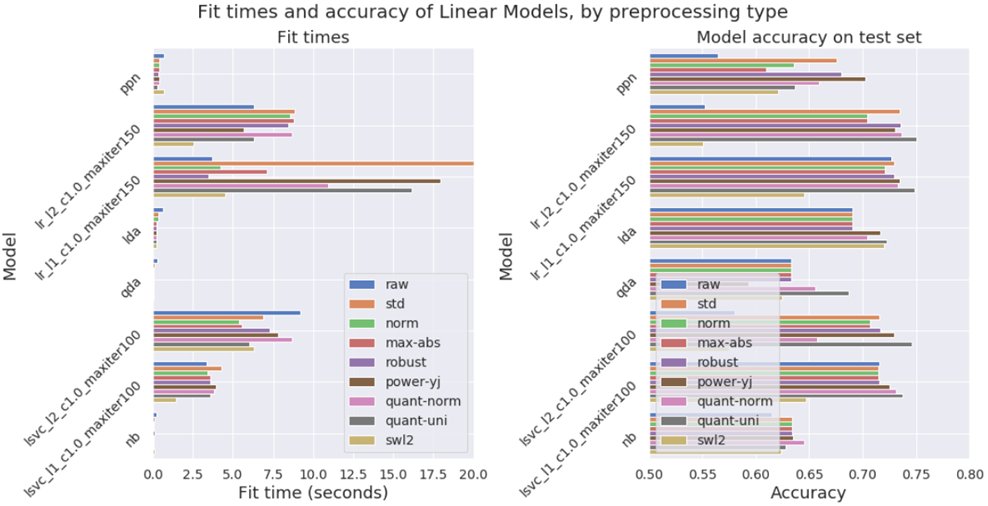
\includegraphics[width=0.98\linewidth,trim=0 0 0 0,clip]{fit_times_linear.png}
        \caption{Fit times and accuracy of linear models, by feature scaling technique.
        Different scaling techniques have a strong effect on the performance of linear models.}
        \label{fig:fit_times_linear}
    \end{figure}

    \item Logistic regression with L2 regularization, regularization parameter $C=0.1$, maximum iterations=100, features transformed with quantile transformation (uniform PDF)

    model code: lr\_l2\_c0.1\_maxiter\_100

    \item Logistic regression with L1 regularization, regularization parameter $C=0.1$, maximum iterations=100, features transformed with quantile transformation (uniform PDF)

    model code: lr\_l1\_c0.1\_maxiter\_100

    \item Linear Discriminant Analysis Classifier, features transformed with quantile transformation (uniform PDF)

    model code: lda

    \item Quadratic Discriminant Analysis Classifier, features transformed with quantile transformation (uniform PDF)

    model code: qda

    \item Linear Support Vector Classification with L2 regularization, regularization parameter $C=0.1$, maximum iterations=100, features transformed with quantile transformation (uniform PDF)

    model code: lsvc\_l2\_c0.1\_maxiter\_100

    \begin{figure}[ht]
        \centering
        \begin{subfigure}{\linewidth}
            \centering
            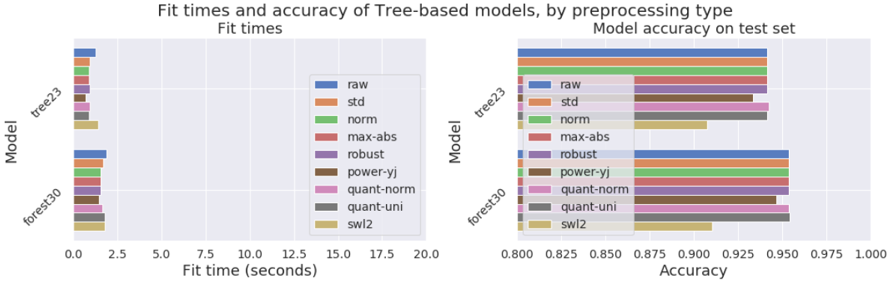
\includegraphics[width=.98\linewidth]{fit_times_trees.png}
            \label{fig:fit_times_trees}
            \caption{Tree-based models: Decision Tree and Random Forest}
        \end{subfigure}

        \begin{subfigure}{\linewidth}
            \centering
            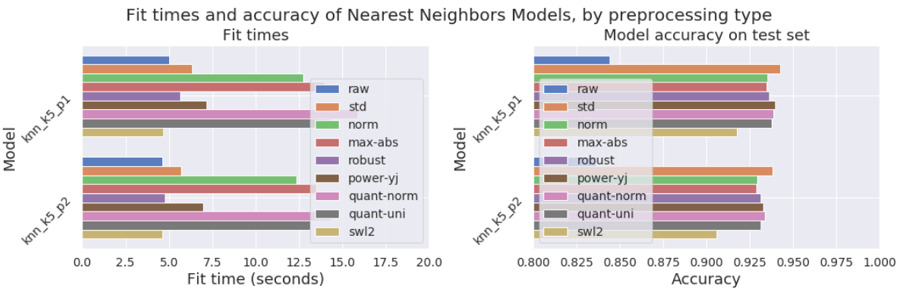
\includegraphics[width=.98\linewidth]{fit_times_neighbors.png}
            \label{fig:fit_times_neighbors}
            \caption{K-Nearest Neighbors: Manhattan and Euclidean distance}
        \end{subfigure}
        \caption{Fit times and accuracy for tree-based models and K-Nearest Neighbors, by feature scaling technique.
        Distance-based algorithms, such as K-Nearest Neighbors are affected by feature scaling, while tree-based models are scale-invariant.}
        \label{fig:fit_times_trees_neighbors}
    \end{figure}

    \item Linear Support Vector Classification with L1 regularization, regularization parameter $C=0.1$, maximum iterations=100, features transformed with quantile transformation (uniform PDF)

    model code: lsvc\_l1\_c0.1\_maxiter\_100

    \item Gaussian Naive Bayes

    model code: nb

    \item Decision Tree, Gini impurity criterion, maximum depth of the tree=25, unscaled features

    model code: tree25

    \item Random Forest, Gini impurity criterion, number of estimators=50, unscaled features

    model code: forest50

    \item K-Nearest Neighbors, Manhattan distance metric, number of neighbors=4, standardized features

    model code: knn\_p1\_k4

\end{itemize}

Different feature scaling techniques have a strong effect on model fit times and predictive performance of linear models, as can be seen on figure~\ref{fig:fit_times_linear}.
Similar to linear models, distance-based algorithms, such as K-Nearest Neighbors, are also strongly affected by feature scaling.
In contrast, tree-based models, such as Decision Tree and Random Forest, are scale-invariant and thus require less preprocessing.
Figure~\ref{fig:fit_times_trees_neighbors} presents fit times for Decision Tree, Random Forest, and K-Nearest Neighbors with Manhattan and Euclidean distance metrics.

\begin{figure}[hbt!]
    \centering
    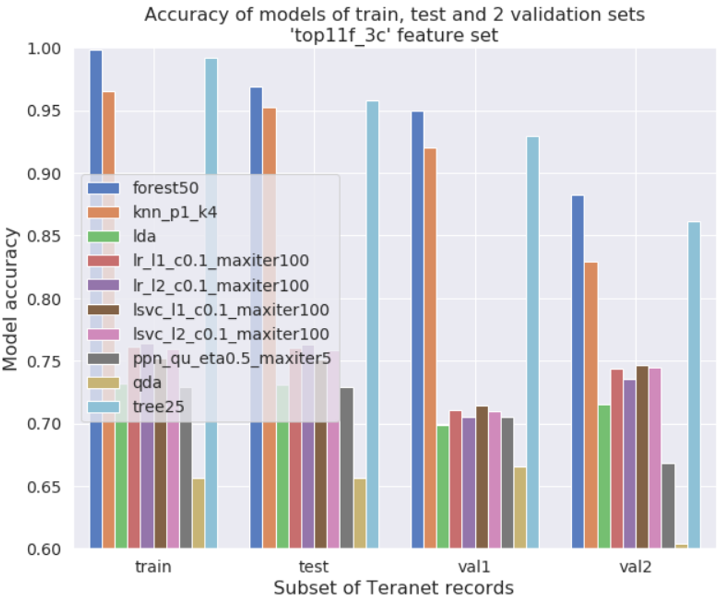
\includegraphics[width=0.6\linewidth,trim=0 0 0 0,clip]{model_performance.png}
    \caption{Model performance (accuracy) on train, test, and two additional validation subsets.
    Additional validation subsets are composed of Teranet records from 2010 and 2015;
    since land use information (target variable) can be less accurate for records in these subsets, they have been used as an additional reference for assessing the generalization of a learning algorithm.}
    \label{fig:model_performance}
\end{figure}

Four different subsets of data have been used to test the best performing models: train, test, and two additional validation subsets.
The train and test subsets represent Teranet records from 2011 to 2014 randomly sampled into 70\% train and 30\% test subsets;
these are the primary subsets that were used for training and tuning the hyperparameters and then evaluating the performance of classifiers on unseen test data, as was described in section~\ref{sec:tuning_hyperparameters}.
The two additional validation subsets were composed of Teranet records from 2010 and 2015.
Since the land use information (target variable) from Department of Geography was collected in 2012 and 2013, it can be less accurate for these subsets;
thus, they have not been used for model selection, training or primary testing, but were utilized to test fitted models as an additional reference for the generalization of performance of classifiers.
Figure~\ref{fig:model_performance} presents model performance on train, test, and two additional validation subsets.

As can be seen on figure~\ref{fig:model_performance}, in terms of prediction accuracy, tree-based and nearest neighbors models dramatically outperform linear models, such as logistic regression, linear SVC, perceptron and LDA classifier.
This indicates that in the current feature space target classes are not linearly separable.
Best-performing linear models were able to reach classification accuracy around 75\% on the test set, with all linear models performing close to each other.
This performance is consistent across the train, test, and both extra validation subsets.
Linear models do not seem to overfit the data, but instead suffer from high bias.

In comparison, tree-based models capable of drawing complex non-linear decision boundaries were able to achieve much higher classification accuracy, with both decision tree and random forest scoring above 95\% on the test set.
These models have a much lower bias on this dataset compared to linear models, but do overfit the training data to some degree under the current size of the training subset.
Validation curve produced during hyperparameter tuning described in section~\ref{sec:tuning_hyperparameters} for decision tree by variating its maximum depth (shown on figure~\ref{fig:validation_tree}) indicates that the model does need to be fairly complex to achieve better classification accuracy;
it suffers from high bias until maximum depth of the tree reaches at least 15.
Then, the model starts to pick up higher variance;
all increases of maximum depth past 23 result mostly in overfitting the training data through unnecessary model complexity and do not yield better generalization.
At a maximum depth of 23, decision tree still has moderate variance, with predictions on the test set being 3\% less accurate then those made on the training data.
Overfitting of the tree also seems to be present on both extra validation subsets, with tree accuracy decreasing further on these subsets;
however, it is challenging to understand whether this is due to the model overfitting training data or due to inaccuracies of target labelling in extra validation subsets.

\begin{figure}[hbt!]
    \centering
    \begin{subfigure}[t]{.47\textwidth}
        \centering
        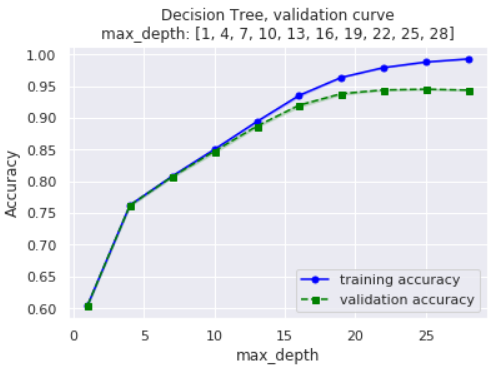
\includegraphics[width=\columnwidth,trim=0 0 0 0,clip]{validation_tree.png}
        \caption{Decision Tree (max\_depth)}
        \label{fig:validation_tree}
    \end{subfigure}
    ~ %add desired spacing between images, e. g. ~, \quad, \qquad, \hfill etc.
    %(or a blank line to force the subfigure onto a new line)
    \begin{subfigure}[t]{.48\textwidth}
        \centering
        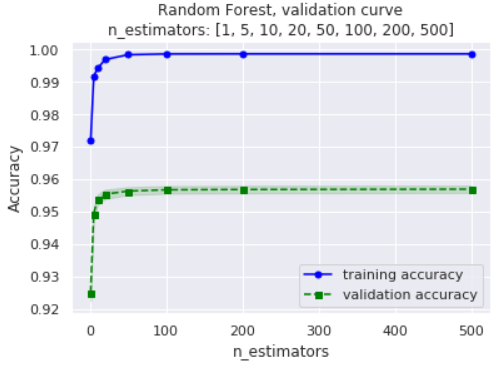
\includegraphics[width=\columnwidth,trim=0 0 0 0,clip]{validation_forest.png}
        \caption{Random Forest (n\_estimators)}
        \label{fig:validation_forest}
    \end{subfigure}
    \caption{Validation curves for decision tree (max\_depth) and Random Forest (n\_estimators) that were produced during model hyperparameter tuning described in section~\ref{sec:tuning_hyperparameters}.}
    \label{fig:validation_curves}
\end{figure}

\begin{figure}[hbt!]
    \centering
    \begin{subfigure}[t]{.47\textwidth}
        \centering
        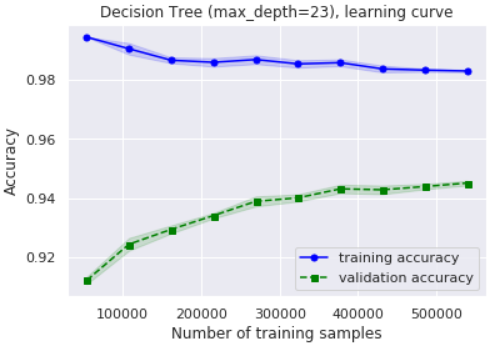
\includegraphics[width=\columnwidth,trim=0 0 0 0,clip]{learning_tree.png}
        \caption{Decision Tree}
        \label{fig:learning_tree}
    \end{subfigure}
    ~ %add desired spacing between images, e. g. ~, \quad, \qquad, \hfill etc.
    %(or a blank line to force the subfigure onto a new line)
    \begin{subfigure}[t]{.48\textwidth}
        \centering
        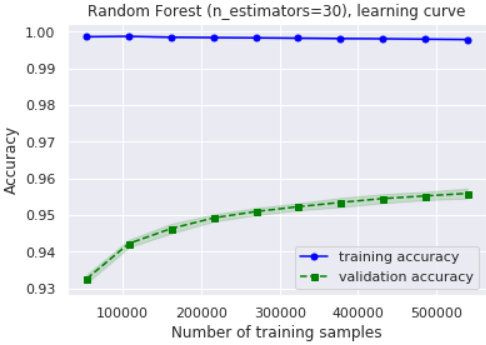
\includegraphics[width=\columnwidth,trim=0 0 0 0,clip]{learning_forest.png}
        \caption{Random Forest}
        \label{fig:learning_forest}
    \end{subfigure}
    \caption{Leaning curves for decision tree and random forest that were produced by variating the size of the training dataset.
    It can be seen that both models overfit training data less with the increase of the training set;
    variance of both models could be reduced further if more data would be used for training.}
    \label{fig:learning_curves}
\end{figure}

Validation curve produced for random forest by variating the number of estimators (presented on figure~\ref{fig:validation_forest}) shows that the model also suffers from some variance and overfits training data.
However, random forest still shows slightly higher prediction accuracy when compared to a single decision tree, and performs better on extra validation subsets.
Since the inaccurate target labelling in extra validation subsets would affect both decision tree and random forest equally, even if it provides a pessimistically biased estimate of algorithm generalization, it can still be used to compare the models between themselves\cite{Raschka2018}.
This indicates that random forest should have better generalization than the decision tree.

Learning curves produced for decision tree and random forest by variating the size of the training set (shown on figure~\ref{fig:learning_curves}) also confirm overfitting of both models.
Their learning curves indicate that variance of both models could be reduced further if more data would be used for training.

$k$-Nearest Neighbors also performs well on test data, with an accuracy slightly lower than that of tree-based models.
It seems to have a low variance between training and test set, but does show stronger decay of performance on both extra validation subsets.
In addition, $k$-NN requires additional preprocessing steps and has much longer fit times on larger datasets when compared with tree-based models;
the computational cost of using a tree to predict data is logarithmic in the number of points used to train the tree.

\section{Best performing model: Random Forest} \label{sec:best_performing_model}

As can be seen from the plots presented in section~\ref{sec:model_performance}, random forest with 50 estimators and Gini impurity criterion showed the best results in terms of accuracy and fit times on all subsets.
Figure~\ref{fig:classification_report_train_test} presents the classification report showing all main model performance metrics for the best performing model: random forest with 50 estimators using Gini impurity criterion.

\begin{figure}[hbt!]
    \centering
    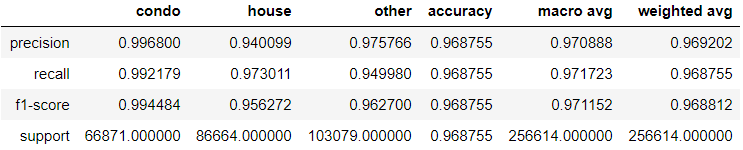
\includegraphics[width=0.98\linewidth,trim=0 0 0 0,clip]{classification_report_train_test.png}
    \caption{Best model performance on test set: classification report for Random Forest with 50 estimators using Gini impurity criterion.}
    \label{fig:classification_report_train_test}
\end{figure}

\begin{figure}[hbt!]
    \centering
    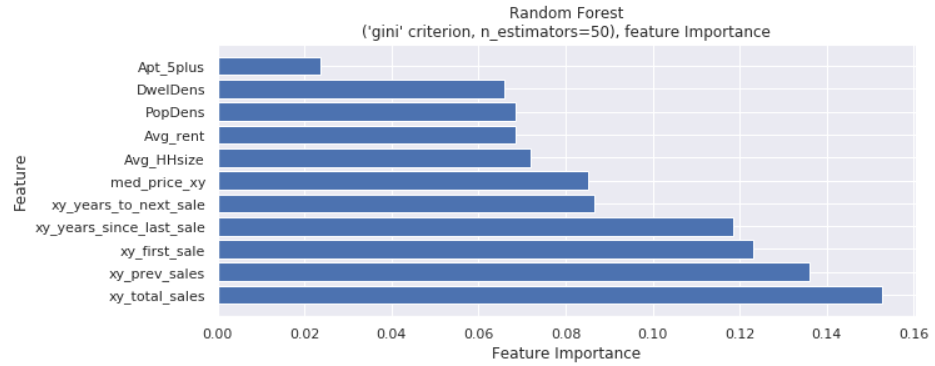
\includegraphics[width=0.95\linewidth,trim=0 0 0 0,clip]{forest_feature_importance.png}
    \caption{Random Forest with 50 estimators using Gini impurity criterion: feature importance.}
    \label{fig:forest_feature_importance}
\end{figure}

Figure~\ref{fig:forest_feature_importance} presents feature importance for the best performing model.
It can be seen that the final random forest model had a fairly balanced use of selected new Teranet and Census variables;
new attributes engineered from native Teranet features that were introduced in section~\ref{sec:feature_engineering} have strong predictive power over land use classes.
It can be seen that the new attributes that relate to the frequency of Teranet records coming from a coordinate pair and new attributes related to time interval between the records from a coordinate pair had the highest importance coefficients for the random forest model.
Census variables that were used to augment Teranet dataset based on relationships that were discussed in chapter~\ref{ch:spatial_and_temporal_relationships} are also related to land use classes and improve the classification accuracy of the model.

Confusion matrices that were introduced in the context of a binary classification problem in section~\ref{sec:model_metrics} can be extended to plot multi-class classification predictions.
Figure~\ref{fig:confusion_matrix_train_test} presents confusion matrices with and without normalization for Random Forest on the test set.

\begin{figure}[hbt!]
    \centering
    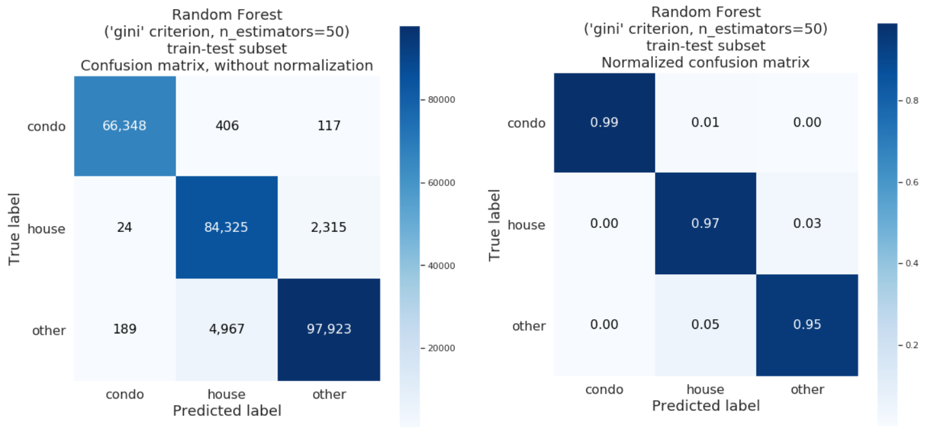
\includegraphics[width=0.98\linewidth,trim=0 0 0 0,clip]{confusion_matrix_train_test.png}
    \caption{Best model performance on test set: confusion matrices with and without normalization for Random Forest with 50 estimators using Gini impurity criterion.
    It can be seen that despite some imbalance in classes, model seems to perform consistently over all three land use categories.}
    \label{fig:confusion_matrix_train_test}
\end{figure}

It can thus be concluded from the classification report (shown on figure~\ref{fig:classification_report_train_test}) and confusion matrices (shown on figure~\ref{fig:confusion_matrix_train_test}) that the model is accurate in its predictions for all three target classes;
moderate class imbalance does not seem to affect accuracy of random forest in classifying the three reduced land use categories.
Thus, this machine learning workflow is capable of producing classification of land use into three major categories (''house'', ''condo'', and ''other'') for each Teranet record starting from 1985;
unbiased performance estimate done on 30\% of held-out test data show 97\% of accuracy for random forest with 50 estimators and Gini impurity criterion.
With further refinement of this workflow, land use can be classified for each Teranet record using newly engineered features and joined Census and TTS variables with a high degree of accuracy.

To facilitate further evaluation of the results produced by this master's thesis and allow ease of access to spatially and temporally related dataset introduced in chapter~\ref{ch:spatial_and_temporal_relationships}, the augmented dataset that was produced as a part of this master's thesis has been saved into a PostgreSQL relational database;
land use produced for each Teranet record by the classification algorithm has been added to augmented Teranet dataset in the database as new feature 'lucr\_predict'.
This way, ease of access and retrieval of this information can be facilitated, as required by the needs of the Longitudinal Analysis of Housing Sales in the GTHA which was introduced in section~\ref{sec:longitudinal_housing_market_research};
in addition, results of this machine learning workflow could be further investigated by a broader and mixed team of specialists.
Entity Relationship (ER) diagram for the database created as a part of this master's thesis is pressented in Appendix~\ref{ch:appendix_rdbms}.

To provide initial EDA of classification errors, counts of Teranet records misclassified by the algorithm by DA have been produced and mapped for the second extra validation subset from 2015 which was showing higher error rates compared to other subsets.
Choropleth (equal interval split of the distribution) map of counts of classification error can be seen on figure~\ref{fig:error_map}.
It can be seen that classification errors are highly localized and likely represent high-frequency transactions corresponding to condo units and mixed use properties.

\begin{figure}[hbt!]
    \centering
    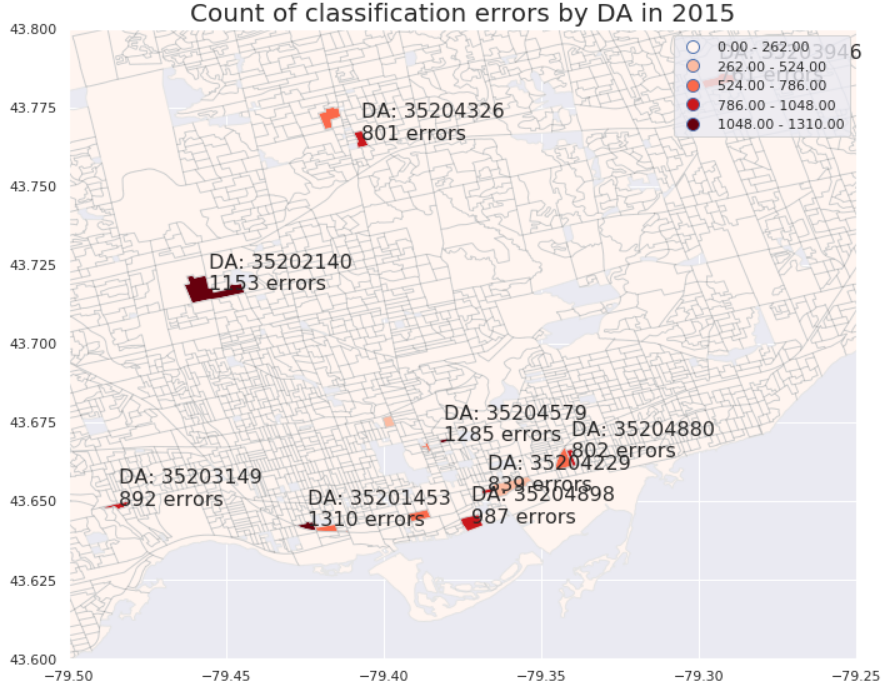
\includegraphics[width=0.8\linewidth,trim=0 0 0 0,clip]{error_map.png}
    \caption{Choropleth (equal interval) map of count of misclassified Teranet records by DA.
    It can be seen that errors are highly localized.}
    \label{fig:error_map}
\end{figure}

\section{Chapter summary} \label{evaluation_summary}

This chapter discussed metrics commonly used to assess performance of classification algorithms, selected criteria for model assessment and acceptance and presented results of model evaluation.
Tree-based models and $k$-Nearest Neighbors significantly outperformed linear models in accuracy;
tree-based models outperformed $k$-NN in fit times.
Learning and validation curves were presented and discussed for tree-based models.
Random forest with 50 estimators was the best performing model and achieved 97\% accuracy on the test set.
Tree-based models have low bias, but do suffer from some overfitting and could benefit from further increase in the size of the training set.
Overall, machine learning workflow introduced by this master's thesis seems to be able to classify land use of Teranet records based on selected features with a high degree of accuracy.
The map of count of classification errors by DA produced from Teranet records from 2015 shows that these errors are highly localized and likely correspond to high-frequency transactions, such as condo units and mixed use properties.
Further investigation of the results of land use classification is required and has been facilitated by transforming the augmented Teranet dataset and other related datasets produced for this master's thesis into a PostgreSQL relational database;
land use predicted by the classification algorithm has been added as a new feature 'lucr\_predict' to each Teranet record within the time span of Census / TTS variables.
Entity Relationship (ER) diagram for the database created as a part of this master's thesis can be found in Appendix~\ref{ch:appendix_rdbms};
its referential integrity constraints were implemented based on the spatial and temporal relationships between data sources that were introduced in chapter~\ref{ch:spatial_and_temporal_relationships}.